\centering
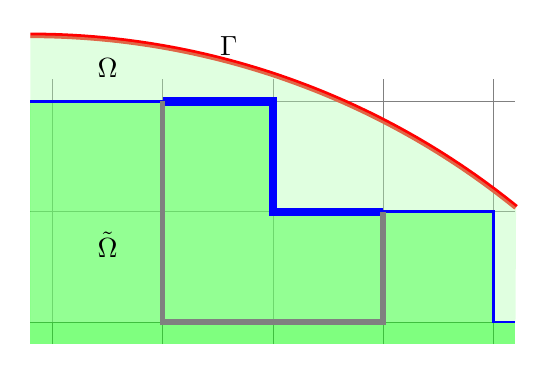
\begin{tikzpicture}[scale=1.4]
    % Draw the Cartesian grid
    \draw[step=1cm, gray, very thin] (0.8,-0.2) grid (5.2,2.2);

    % Highlight cells inside the domain (interior cells)
    \foreach \x/\y in {2/1, 1/0, 1/1, 2/0, 3/0, 4/0}
        {
            \fill[green, opacity=0.5] (\x,\y) rectangle (\x+1,\y+1);
        }
    \foreach \x/\y in {1/0 }{
            \fill[green, opacity=0.5] (\x,\y) rectangle (\x-0.2,\y+2);
        }

    \fill[green, opacity=0.5] (0.8,-0.2) rectangle (5.2,0);

    \draw[line width=2pt, red, domain=51:90, samples=100, variable=\t]
    plot ({0.8 + 7.0*cos(\t)}, {-4.4 + 7.0*sin(\t)});
    \node at (2.6,2.5) {$\Gamma$};

    % Fill the area below the red line with light green to indicate the domain Omega
    \fill[green!30, opacity=0.4] plot[domain=51:90, samples=100, variable=\t] ({0.8 + 7.0*cos(\t)}, {-4.4 +
            7.0*sin(\t)}) -- (0.8,0) -- (5.2,0) -- cycle;

    % Draw the surrogate boundary (only the top boundary of the interior cells)
    \draw[line width=1pt, blue] (0.8,2) -- (3,2) -- (3,1) -- (4,1) -- (5,1)-- (5,0)-- (5.2,0.) ;

    % Draw the surrogate boundary in the single patch case
    \draw[line width=3pt, blue] (2,2) -- (3,2) -- (3,1) -- (4,1);

    % Draw the interior boundary 
    \draw[line width=2pt, gray] (2,2) -- (2,0) -- (4,0) -- (4,1);

    \node at (1.5,0.7) {$\tilde{\Omega}$};

    \node at (1.5,2.3) {${\Omega}$};

\end{tikzpicture}
